\subsection*{Funciones Generadoras Ordinarias}

%\fcolorbox{cyan}{red}{Documento en construcción}

\subsubsection*{Descripción}
Una función generadora es una serie de potencias cuyos coeficientes corresponden a los términos de una secuencia. De este modo, las secuencias pueden ser definidas mediante una función generadora, lo que a su vez significa que permiten transformar problemas con secuencias en problemas con funciones.

Dada una secuencia $\langle f(0),\,f(1),\,f(2),\,..f(n),\,...\rangle$, se define su función generadora como
\begin{equation}
    \label{eq:gen-function}
    F(z) = \sum_{n\ge 0}{{\color{blue}f(n)}\cdot{\color{red}z^n}} 
    = {\color{blue}f(0)}\cdot \color{red}z^0 + {\color{blue}f(1)}\cdot \color{red}z^1 + {\color{blue}f(2)}\cdot \color{red}z^2 + \cdots + {\color{blue}f(n)}\cdot \color{red}z^n + \cdots  
\end{equation}

En \eqref{eq:gen-function} se observa que se están tomando todos los términos de la secuencia, que son infinitos, y que cada $n$-ésimo término, de la secuencia, está multiplicado por la $n$-ésima potencia de $z$. El término $f(n)$ representa todos los términos de la secuencia, quienes en la función generadora, pasan a ser los coeficientes. \textbf{De modo que una vez se tiene la función generadora de una secuencia, es posible hallar la fórmula para la secuencia a partir del hallazgo de los coeficientes de la función generadora}.\\


Por ejemplo dada la secuencia de unos, donde $f_n = 1$, es decir, todos los términos de la secuencia son $1$, su función generadora será

\begin{equation}
    \label{eq:gf-1-seq-basic}
    F(z) = \sum_{n\ge 0}{ 1\cdot z^n} =1\cdot z^0 + 1\cdot z^1 + 1\cdot z^2 + \cdots +  1\cdot z^n + \cdots 
\end{equation}

Esta función generadora, corresponde a una serie geométrica donde el radio es igual a 1, y converge a un valor que corresponde a 

\begin{equation}
    F(z) = \sum_{n\geq0}{1\cdot z^n} = \frac{1}{1-z}.
\end{equation}

Si en lugar de una secuencia $\langle 1\rangle_{n\ge 0}$, se tuviera la secuencia de los enteros no negativos, es decir, $\langle n\rangle_{n\ge 0}$, la función generadora sería:

\begin{equation}
    \label{eq:gf-N-seq-basic}
    F(z)= \sum_{n\geq0}{n \cdot z^n} = 0 + 1\cdot z^1 + 2\cdot z^2 + \cdots +  n\cdot z^n + \cdots 
\end{equation}

Al igual que la ecuación \eqref{eq:gf-1-seq-basic}, esta función generadora converge a un valor

\begin{equation}
    F(z)= \sum_{n\geq0}{n\cdot z^n} = \frac{z}{(1-z)^2}
\end{equation}

Es importante resaltar que en lo relacionado a funciones generadoras, $F(z)$, el objetivo es hallar los coeficientes, $f(n)$, a partir de una función generadora dada, y para ello se recurre a las funciones generadoras básicas (ver Tabla 1) y a las operaciones básicas (ver Tabla 2) relacionadas con estas.\\

La forma utilizada para describir la relación descrita es:
\begin{align*}
    F(z)&\texttt{ Es la FGO de la secuencia }f(n).
\end{align*}
Claramente, esto significa que
\begin{align*}
    F(z)=\sum_{n\geq0}{f(n)\cdot z^n} & \texttt{ Es la FGO de la secuencia } \langle f(n) \rangle_{n\ge 0}.
\end{align*}
Por ejemplo:
\begin{align*}
    F(z)=\dfrac{1}{1-z}&\texttt{ Es la FGO de la secuencia }f(n)=\langle 1 \rangle_{n\ge 0}.
\end{align*}
\newpage
\renewcommand{\arraystretch}{2}

\begin{table}[t]
\begin{tabularx}{\linewidth}{X}
\end{tabularx}
\label{tab:ogf-basic}
\begin{align*}
    &\langle 1,\, 1,\, 1,\,\dots,\,1,\,\dots \rangle
    &
    \frac{1}{1-z} &= \sum_{n\geq0}{z^n}
    \\
    &\langle 0,\,1,\,2,\,3,\,\dots,\,n,\,\dots \rangle
    &
    \frac{z}{(1-z)^2} &= \sum_{n\geq0}{nz^n}
    \\
    &\left\langle 0,\,0,\,1,\,3,\,6,\,\dots, \binom{n}{2}, \dots \right\rangle
    &
    \frac{z^2}{(1-z)^3} &= \sum_{n\geq2}{\binom{n}{2}z^n}
    \\
    &\left\langle 0,\,\dots,\,0,\,1,\,m+1,\,\dots,\,\binom{n}{m}, \dots \right\rangle
    &
    \frac{z^m}{(1-z)^{m+1}} &= \sum_{n\geq m}{\binom{n}{m}z^n}
    \\
    &\left\langle 1,\,m+1,\,\binom{m+2}{2},\,\binom{m+3}{3},\,\dots,\,\binom{n}{m}, \dots \right\rangle
    &
    \frac{1}{(1-z)^{m}} &= \sum_{n\geq 0}{\binom{n+m-1}{m}z^n}
    \\
    & \langle 1,\, 0,\, 1,\,\dots,\,1,\,0,\,\dots \rangle
    &
    \frac{1}{1-z^2} &= \sum_{n\geq0}{z^{2n}}= \sum_{n\geq0}\left(\frac{1+(-1)^n}{2}\right) z^{n}
    \\
    & \langle 2^0,\, 2^1,\, 2^2,\,2^3,\,\dots,\,2^n,\,\dots \rangle
    &
    \frac{1}{1-2z} &= \sum_{n\geq0}{2^n\cdot z^{n}}= \sum_{n\geq0}(2 \cdot z)^n
    \\
    & \langle c^0,\, c^1,\, c^2,\,c^3,\,\dots,\,c^n,\,\dots \rangle
    &
    \frac{1}{1-cz} &= \sum_{n\geq0}{c^nz^{n}}
    \\
    & \left\langle \binom{m}{0},\,\binom{m}{1},\,\dots,\,\binom{m}{n},\,\dots,\,
    ,\,\binom{m}{1},\,\binom{m}{0} \right\rangle.
    &
    \left(1+z\right)^m &= \sum_{n\geq0}{\binom{m}{n}z^n}
    \\
    & \left\langle 0,\, 1,\,\cfrac{1}{2},\,\cfrac{1}{3},\,\dots,\,
    \,\cfrac{1}{n},\,\dots \right\rangle
    &
    \ln{\left(\cfrac{1}{1-z}\right)} &= \sum_{N\geq1}{\cfrac{z^n}{n}}
\end{align*}
\caption{Algunas Funciones Generadoras Básicas}
\end{table}

En la Tabla 1 se muestran algunas funciones generadoras básicas y que mediante su manipulación, permiten hallar los coeficientes de otras funciones generadoras. Estas manipulaciones se realizan mediante el uso de las operaciones definidas para las funciones generadoras.

\begin{table}[ht!]
\begin{tabularx}{\linewidth}{X X X X}
    {Suma  (o resta) \newline $$F(z)+G(z)$$}
    & $$\sum_{n\geq0}{(f(n) + g(n))\cdot z^n}$$ 
    & $$f(0) + g(0),\, f(1) + g(1),\,\dots,\,f(n)+g(n),\,\dots$$
    \\
    {Escala \newline $$F(k\cdot z)$$} 
    & $$\sum_{n\geq0}{f(n)\cdot k^n\cdot z^n}$$ 
    & $$f_0,kf_1,k^2f_2,\,\dots,\,k^nf_n,\,\dots$$
    \\
    {Derivada \newline $$F'(z)$$}
    & $$\sum_{n\geq0}{(n+1)\cdot f_{n+1}\cdot z^{n}}$$
    & $$f_1,\,2\cdot f_2,\,3\cdot f_3,\,\dots,n\cdot f_n\,\dots$$
    \\
    {Suma Parcial \newline $$\cfrac{F(z)}{1-z}$$}
    & $$\sum_{n\geq0}{\left(
        \sum_{0\leq k\leq n}{f_k}
    \right)z^n}$$
    &  $$f_0,\,f_0+f_1,\dots,\,\sum_{0\leq k \leq n}{f_k},\dots$$
    \\
    {Convolución  \newline $$F(z) \cdot G(z)$$}
    & $$\sum_{n\geq0}{\left(\sum_{0\leq k \leq n}{f_k\cdot g_{n-k}}\right)z^n}$$ 
    & $$f_0g_0,\,f_1g_0+f_0g_1,
    \,\dots,\sum_{0\leq k\leq n}{f_k\cdot g_{n-k}}$$ \\
    {Desplazar a la derecha \newline $$z\cdot F(z)$$}
    & $$\sum_{n\geq1}{f(n-1)\cdot z^n}$$
    & $0,\,f_0,\,f_1,\,f_2,\dots,f_n,\dots$
    \\
    {Diferencia (Telescópica) \newline $$(1-z)\cdot F(z)$$}
    & $$f(0) + \sum_{n\geq1}{(f_n - f_{n-1})\cdot  z^n}$$
    & $$f_0,\,f_1-f_0,\dots,f_n-f_{n-1},\dots$$
\end{tabularx}
\caption{Operaciones básicas con Funciones Generadoras}
\label{tab:ogf-basic-ops}
\end{table}

\clearpage

El procedimiento general para hallar la función generadora $F(z)$ de una secuencia $\seq{f(n)}{0}$ es el de primero definir $F(z)$, esto es:
\begin{align*}
    F(z)&=\sum_{n\geq0}{f(n)\cdot z^n}.
\end{align*}

A partir de aquí, hay varias maneras de proceder:

\begin{itemize}
    \item Una posible opción es la de modificar esta expresión de $F(z)$ utilizando las propiedades de las OGF para así llegar a las OGF básicas, de modo que $F(z)$ finalmente quede en función de estas. 
    \item También es posible empezar con una OGF básica e ir aplicando distintas propiedades a estas hasta llegar a la expresión de la sumatoria de $F(z)$.
\end{itemize}
\subsubsection*{Ejemplos}
\paragraph{Ejemplo 1} Dada la secuencia $\seq{2^{n+1}}{2}$, halle su función generadora.

Este ejemplo lo resolveremos usando una de las funciones generadoras básicas y aplicando propiedades sucesivamente hasta llegar a la expresión buscada.

Lo primero es definir lo siguiente:

Dada la secuencia $\seq{\cmag{2^{n+1}}}{\cyan{2}}$, definimos $F(z)$ como su función generadora.
\begin{align*}
    F(z)&=\sum_{\cyan{n\geq2}}{\cmag{2^{n+1}}\cdot z^n}.
\end{align*}

Empezaremos usando la OGF más básica:
\begin{align*}
    \cfrac{1}{1-z}&=\sum_{n\geq0}{z^n}.
\end{align*}
El procedimiento a seguir es aplicar propiedades de las OGF hasta que el lado derecho de la ecuación sea igual al buscado, es decir, la expresión de la sumatoria en $F(z)$.

Primero aplicaremos la propiedad de escala, con $k=2$:
\begin{align*}
    \cfrac{1}{1-\cmag{2}z}&=\sum_{n\geq0}{\cmag{2^n}\cdot z^n}.
\end{align*}
Ahora, dado que la expresión buscada tiene $2^{n+1}$, multiplicamos ambos lados de la expresión por 2.
\begin{align*}
    2\cdot\left(\cfrac{1}{1-2z}\right)&=2\cdot\left(\sum_{n\geq0}{2^n\cdot z^n}\right)\\
    \cfrac{2}{1-2z}&=\sum_{n\geq0}{2^{n+1}\cdot z^n}
\end{align*}
La expresión de la sumatoria es muy cercana a la buscada, sin embargo, aún falta el índice de la sumatoria en la expresión que buscamos. Por lo tanto, separamos la sumatoria.

Para aclarar lo que se hará, es importante recordar la definición de FGO:
\begin{equation*}
    \label{eq:gen-function1}
    \sum_{n\ge 0}{{\color{blue}f(n)}\cdot{\color{red}z^n}} 
    = {\color{blue}f(0)}\cdot \color{red}z^0 + {\color{blue}f(1)}\cdot \color{red}z^1 + {\color{blue}f(2)}\cdot \color{red}z^2 + \cdots + {\color{blue}f(n)}\cdot \color{red}z^n + \cdots  
\end{equation*}
y que esto puede ser reescrito de diversas maneras, y en este caso, usando la propiedad asociativa de la suma, tenemos:
\begin{align*}
    \sum_{n\geq0}{f(n)\cdot z^n} &= \cyan{\left(f(0) + f(1)\cdot z^1\right)} + \cmag{\left(f(2)\cdot z^2 + f(3)\cdot z^3 + \cdots \right)}\\
    \sum_{n\geq0}{f(n)\cdot z^n} &=\cyan{\sum_{0\leq n \leq 1}{f(n)\cdot z^n}} + \cmag{\sum_{n\geq2}{f(n)\cdot z^n}}
\end{align*}
nos será bastante útil. Dado que ahora reescribimos
\begin{align*}
    \cfrac{2}{1-2z}&=\sum_{n\geq0}{2^{n+1}\cdot z^n}
\end{align*}
como
\begin{align*}
    \cfrac{2}{1-2z}&=\sum_{0\leq n\leq 1}{2^{n+1}\cdot z^n}+\underbset{F(z)}{\sum_{n\geq2}{2^{n+1}\cdot z^n}}.
\end{align*}
A partir de aquí, ya que tenemos $F(z)$, lo que hacemos es despejar.
\begin{align*}
    \cfrac{2}{1-2z}&=\sum_{0\leq n\leq 1}{2^{n+1}\cdot z^n}+F(z)\\
    F(z)&=\cfrac{2}{1-2z}-\sum_{0\leq n\leq 1}{2^{n+1}\cdot z^n}\\
    F(z)&=\cfrac{2}{1-2z}-2^2\cdot z^1 - 2^1\cdot z^0\\
    F(z)&=\cfrac{2}{1-2z}-4z-2.
\end{align*}
De aquí, tenemos que la respuesta es que la función generadora de la secuencia $\seq{2^{n+1}}{2}$ es 
$$F(z)=\cfrac{2}{1-2z}-4z-2.$$

\paragraph{Ejemplo 2}
Dada la siguiente secuencia $\seq{f(n)}{0}$, halle su OGF.
\begin{align*}
    f_n&=\begin{cases}
    \cyan{n,\quad n\geq4}\\
    \cmag{1,\quad 1\leq n < 4}\\
    0,\quad n=0
    \end{cases}
\end{align*}
Primero, definimos $F(z)$ como la función generadora de la secuencia $f(n)$
\begin{align*}
    F(z)&=\cmag{\sum_{1\leq N\leq 3}{1\cdot z^N}} + \cyan{\sum_{n\geq 4}{n\cdot z^n}} \color{gray!35}+ 0\cdot z^0
\end{align*}
Este ejemplo lo resolveremos usando, nuevamente, la OGF más básica. Es importante resaltar que se puede empezar a partir de cualquier otra de las OGF, pero utilizamos esta para así mostrar más ejemplos de las operaciones.
\begin{align*}
    \cfrac{1}{1-z}&=\sum_{n\geq0}{z^n}.
\end{align*}
Primero procedemos a aplicar la operación de multiplicación por el índice a la función generadora. Por lo que al aplicar la operación siguiendo su definición en la tabla, obtenemos:
\begin{align*}
    \cfrac{1}{(1-z)^2}&=\sum_{n\geq0}{(n+1)\cdot z^n}.
\end{align*}
Aquí podemos bien o aplicar el cambio de variable $n\xrightarrow{} n-1$ en la sumatoria o bien, aplicar la operación de desplazar a la derecha [la secuencia]. En todo caso, el resultado es el mismo:
\begin{align*}
    \cfrac{z}{(1-z)^2}&=\sum_{n\geq0}{n\cdot z^n} \cmag{\left(=\sum_{n\geq1}{n\cdot z^n}\right)}.
\end{align*}
Esta expresión ya es más cercana a la que buscamos. Sin embargo, el índice de esta sumatoria inicia en 0, y el buscado inicia en 4, por lo que procedemos a restar estos elementos:
\begin{align*}
    \cfrac{z}{(1-z)^2}&=\sum_{n\geq0}{n\cdot z^n}\\
    &=\sum_{0\leq n\leq3}{n\cdot z^n}+\sum_{n\geq4}{n\cdot z^n}\\
    \cfrac{z}{(1-z)^2}-\sum_{0\leq n\leq3}{N\cdot z^n}&=\sum_{n\geq4}{n\cdot z^n}\\
    \cfrac{z}{(1-z)^2}-3z^3-2z^2-z&=\sum_{n\geq4}{n\cdot z^n}.
\end{align*}
Luego de este paso, vemos que aún falta la otra sumatoria de la definición de $F(z)$ para este ejercicio. Por lo que simplemente sumamos la expresión de ambos lados y obtenemos:
\begin{align*}
    \cfrac{z}{(1-z)^2}-3z^3-2z^2-z+\cyan{\sum_{1\leq n\leq 3}{1\cdot z^n}}&=\underbset{F(z)}{\sum_{n\geq4}{n\cdot z^n}+\cyan{\sum_{1\leq n\leq 3}{1\cdot z^n}}},
\end{align*}
y aquí una vez más ya tenemos nuestro $F(z)$.
\begin{align*}
    F(z)&=\cfrac{z}{(1-z)^2}-3z^3-2z^2-z+\cyan{\sum_{1\leq n\leq 3}{1\cdot z^n}}\\
    &=\cfrac{z}{(1-z)^2}-3z^3-2z^2-z+\cyan{z+z^2+z^3}\\
    F(z)&=\cfrac{z}{(1-z)^2}-2z^3-z^2.
\end{align*}
Por lo que finalmente la solución a este ejemplo es que la OGF de la secuencia 
\begin{align*}
    f_n&=\begin{cases}
    n,\quad n\geq4\\
    1,\quad 1\leq n < 4\\
    0,\quad n=0
    \end{cases}
\end{align*}
es
\begin{align*}
F(z)&=\cfrac{z}{(1-z)^2}-2z^3-z^2.
\end{align*}
\clearpage
\section{Entregable 01}
\section*{Problema 1: Funciones Generadoras y Secuencias.}

Encuentre una forma cerrada para la función generadora ordinaria, $F_i(z)$, para cada una de las siguientes secuencias $\langle f(n) \rangle_{n\ge n_0}$:
\label{sec:ogf-seq}
\begin{flushleft}
    \fcolorbox{blue}{white}{\large \bf \textcolor{blue}{Importante}}
\end{flushleft}
Para cada problema, excepto el número 2, el equipo tiene que hallar:

\begin{itemize}
    \item La versión NO recurrente de $f(n)$ 
    \item Una de las versiones recurrentes de $f(n)$ 
    \item La FGO
    \item Graficar la NO recurrente y la FGO, 1000 primeros valores
\end{itemize}
\begin{enumerate}
     \item\,[*] Sea $f(n)$ el número de subconjuntos, del conjunto $S=\{1, 2,...,n\}$, que no contienen dos enteros consecutivos.
     \\
     
\includegraphics[width= 10 mm]{figures/exc.png}\textbf{(Estudiante Alejandra Landinez Lamadrid - 200161946)}
     \begin{itemize}
         \item Versión \textbf{NO} recurrente de $f(n)$: 
         \\
         Utilizamos la fórmula de serie geométrica:\\ 
         \\
         $\frac{1}{1-x} = \sum_{n=0} x^n$\\
         \\
         $x = -z-z^2$\\
         \begin{align*}
             \frac{1}{1+z+z^2} &= \sum_{n=0} (-z-z^2)^n\\
             &= \sum_{n=0} \binom{-n}{n}(-1)^n\cdotz^n\cdot(1+z)^n\\
             &= \sum_{n=0} (-1)^n\cdot \binom{2n-1}{n}\cdot z^n (1+z)^n\\
             f(n) &= (-1)^n \cdot \binom{2n-1}{n}
         \end{align*}
         \item Versión recurrente de $f(n): f(n-1)+f(n-2)$
         \\
         \item FGO:
         \\
         \begin{align*} 
         F(z) &=\sum_{n\geq0} f(n)\cdot z^n\\
         &=\sum_{n\geq0} (f(n-1)+f(n-2))\cdot z^n\\
         &=\sum_{n\geq0} f(n-1)\cdot z^n + \sum_{n\geq0} f(n-2)\cdot z^n\\
         &=\sum_{n\geq1} f(n)\cdot z^n + \sum_{n\geq2} f(n)\cdot z^n\\
         \end{align*}
         Factorizamos las sumatorias:
         \begin{align*}
             \sum_{n\geq1} f(n)\cdot z^n = z\cdot \sum_{n\geq1} f(n)\cdot z^{n-1} = z\cdot F(z)\\
             \sum_{n\geq2} f(n)\cdot z^n = z^2\cdot \sum_{n\geq2} f(n)\cdot z^{n-2} = z^2\cdot F(z)
         \end{align*}\\
         Reemplazamos los términos factorizados:
         \begin{align*}
             F(z) &= z\cdot F(z) + z^2\cdot F(z)\\
             &= z\cdot F(z)\cdot (1+z)\\
             F(z) &= \frac{1}{1-z-z^2}
         \end{align*}
         \cite{chatGPT_FGO}
         \\Gráficas FGO y f(n)\\
         \begin{center}
         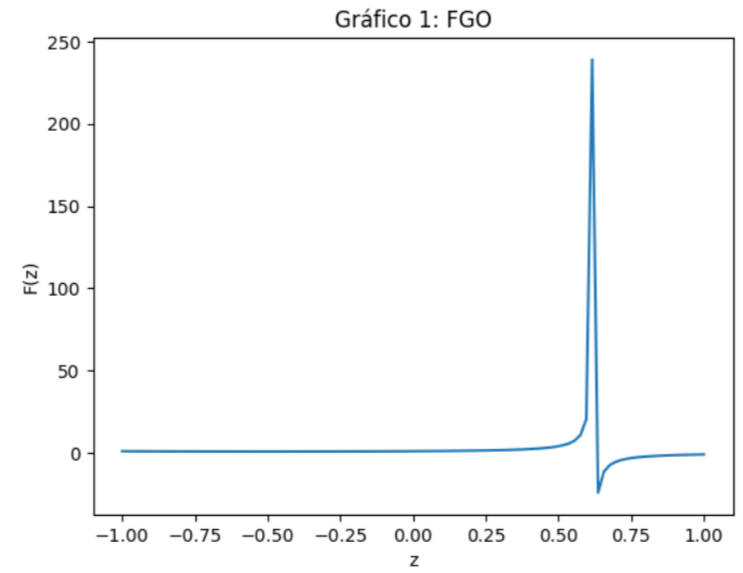
\includegraphics[width= 90 mm]{imagenes-gráficas/fgo_1.png}
         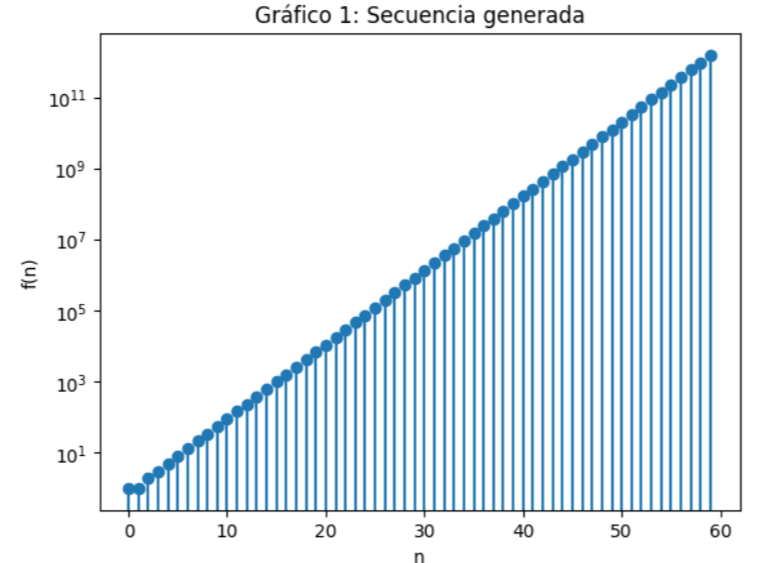
\includegraphics[width= 90 mm]{imagenes-gráficas/secuencias_1.png}
         \end{center}
     \end{itemize} 
     
    \item\,[*] Sea $f(n)$ el número de particiones de un conjunto de n elementos. \\
    La solución a este problema fue desarrollada por Eric Temple Bell. El $n$-ésimo número de Bell está definido por: $$B(n+1)=\sum_{i=0}^{n}\dbinom{n}{i}\cdot B(i)$$
    Ejemplo, para $B(3)=5$ las particiones son: 
    \begin{itemize}
        \item $\{\; \{1\}\cup \{2\}\cup \{3\}\; \}$
        \item $\{\; \{1, 2\}\cup \{3\} \;\} $
        \item $\{\; \{1, 3\}\cup \{2\}\; \}$
        \item $\{\; \{2, 3\}\cup \{1\}\; \}$
        \item $ \{1, 2, 3\} $
    \end{itemize}
    Imprima la secuencia de los números de Bell e ilustre, como en el ejemplo anterior $B(n),\, n=0,1,2,3,4$ y $5$ 

    
\includegraphics[width= 10 mm]{figures/exc.png}\textbf{(Estudiante Mariana Guerrero Benavides-200173479)}
    
    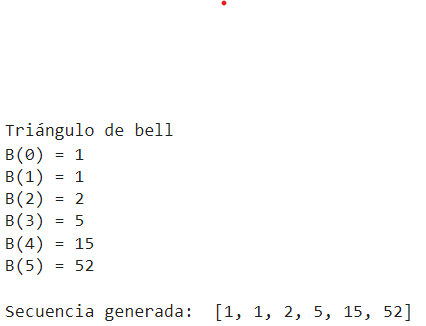
\includegraphics[width=.4\textwidth,height=.4\textwidth]{figures/Secuencia_Num_Bell.png}
    \begin{itemize}
        \item Para \colorbox{yellow}{$B(0)=1$}

        Particiones: $\{ \{\}\}$
        \item Para $n=0$ $$B(0+1)=\dbinom{0}{0}\cdot B(0) =1$$

        \colorbox{yellow}{$B(1)=1$}

        Particiones: $\{ \{1\}\}$
        \item  Para $n=1$ $$B(1+1)=\dbinom{1}{0}\cdot B(0) + \dbinom{1}{1} \cdot B(1)=$$

        $$B(2)= 1+1 = 2$$

        \colorbox{yellow}{$B(2)=2$}

        Particiones: 
            \begin{itemize}
                \item $\{\; \{1\}\cup \{2\} \}$
                \item $\{\; \{1, 2\}\} $
            \end{itemize}
        \item Para $n=2$ $$B(2+1)=\dbinom{2}{0}\cdot B(0) + \dbinom{2}{1} \cdot B(1) + \dbinom{2}{2} \cdot B(2)=$$

        $$B(3)= B(0) + 2B(1) + B(2) = 1 + 2 \cdot 1 + 2 =$$

        \colorbox{yellow}{$B(3)=5$}
        Particiones: 
            \begin{itemize}
                \item $\{\; \{1\}\cup \{2\} \cup \{3\}\}$
                \item $\{\; \{1, 2, 3\}\} $
                \item $\{\; \{1, 2\} \cup \{3\}\}$
                \item $\{\; \{1, 3\} \cup \{2\}\}$
                \item $\{\; \{2, 3\} \cup \{1\}\}$
            \end{itemize}
            
        \item Para $n=3$ $$B(3+1)=\dbinom{3}{0}\cdot B(0) + \dbinom{3}{1} \cdot B(1) + \dbinom{3}{2} \cdot B(2)+ \dbinom{3}{3} \cdot B(3)=$$

        $$B(4)= B(0) + 3B(1) + 3B(2) + B(3)= 1 + 3 \cdot 1+  3 \cdot 2 + 5 =$$

        \colorbox{yellow}{$B(4)=15$}
        Particiones: 
            \begin{itemize}
                \item $\{\; \{1\}\cup \{2\} \cup \{3\} \cup \{4\}\}$
                \item $\{\; \{1, 2, 3, 4\}\} $
                \item $\{\; \{1\}\cup \{2,3,4\}\}$
                \item $\{\; \{2\} \cup \{1,3,4\}\}$
                \item $\{\; \{3\} \cup \{1,2,4\}\}$
                \item $\{\; \{4\} \cup \{1,2,3\}\}$
                \item $\{\; \{1,2\} \cup \{3,4\}\}$
                \item $\{\; \{1,3\} \cup \{2,4\}\}$
                \item $\{\; \{1,4\} \cup \{2,3\}\}$
                \item $\{\; \{1,2\} \cup \{3\} \cup \{4\} \}$
            \item $\{\; \{1,3\} \cup \{2\} \cup \{4\} \}$
                \item $\{\; \{1,4\} \cup \{2\} \cup \{3\} \}$
                \item $\{\; \{2,3\} \cup \{1\} \cup \{4\} \}$
                \item $\{\; \{2,4\} \cup \{1\} \cup \{3\} \}$
                \item $\{\; \{3,4\} \cup \{1\} \cup \{2\} \}$
            \end{itemize}
        
        \item Para $n=4$ $$B(4+1)=\dbinom{4}{0}\cdot B(0) + \dbinom{4}{1} \cdot B(1) + \dbinom{4}{2} \cdot B(2)+ \dbinom{4}{3} \cdot B(3) + \dbinom{4}{4} \cdot B(4)=$$

        $$B(5)= B(0) + 4B(1) + 4B(2) + 4B(3) + B(4)= 4 \cdot 1 + 4 \cdot 1+  4 \cdot 2 + 4 \cdot 5 + 15 =$$

        \colorbox{yellow}{$B(5)=52$}
        Particiones: 
            \begin{itemize}
                \item $\{\; \{1\}\cup \{2\} \cup \{3\} \cup \{4\} \cup \{5\}\}$
                \item $\{\; \{1, 2, 3, 4, 5\}\} $
                \item $\{\; \{1,2\} \cup \{2,3\} \cup \{3,4\} \cup \{4,5\}\}$
                \item $\{\; \{1,3\} \cup \{2,4\} \cup \{5\}\}$
                \item $\{\; \{1,3\} \cup \{2,5\} \cup \{4\}\}$
                \item $\{\; \{1,3\} \cup \{4,5\} \cup \{2\}\}$
                \item $\{\; \{1,4\} \cup \{2,5\} \cup \{3\}\}$
                \item $\{\; \{1,4\} \cup \{2,3\} \cup \{5\}\}$
                \item $\{\; \{1,4\} \cup \{3,5\} \cup \{2\}\}$
                \item $\{\; \{1,5\} \cup \{3,4\} \cup \{2\}\}$
                \item $\{\; \{1,5\} \cup \{2,3\} \cup \{4\}\}$
                \item $\{\; \{1,5\} \cup \{2,4\} \cup \{3\}\}$
                \item $\{\; \{1,2\} \cup \{3,4\} \cup \{5\}\}$
                \item $\{\; \{1,2\} \cup \{3,5\} \cup \{4\}\}$
                 \item $\{\; \{1,2\} \cup \{4,5\} \cup \{3\}\}$
                \item $\{\; \{1\} \cup \{2,3,4,5\}\}$
                \item $\{\; \{2\} \cup \{1,3,4,5\}\}$
                \item $\{\; \{3\} \cup \{1,2,4,5\}\}$
                \item $\{\; \{4\} \cup \{1,2,3,5\} \}$
                \item $\{\; \{5\} \cup \{1,2,3,4\} \}$
                \item $\{\; \{1,2\} \cup \{3,4,5\} \}$
                \item $\{\; \{1,3\} \cup \{2,4,5\} \}$
                \item $\{\; \{1,4\} \cup \{2,3,5\} \}$
                \item $\{\; \{1,5\} \cup \{2,3,4\}  \}$
                \item $\{\; \{1\}\cup \{2\} \cup \{3,4,5\} \}$
                \item $\{\; \{1\}\cup \{3\} \cup \{2,4,5\} \}$
                \item $\{\; \{1\}\cup \{4\} \cup \{2,3,5\} \}$
                \item $\{\; \{1\}\cup \{5\} \cup \{2,3, 4\} \}$
                \item $\{\; \{2,3\} \cup \{1,4,5\} \}$
                \item $\{\; \{2,4\} \cup \{1,3,5\} \}$
                \item $\{\; \{2,5\} \cup \{1,3,4\} \}$
                \item $\{\; \{2\}\cup \{3\} \cup \{1,4,5\} \}$
                \item $\{\; \{2\}\cup \{4\} \cup \{1,3,5\} \}$
                \item $\{\; \{2\}\cup \{5\} \cup \{1,3,4\} \}$
                \item $\{\; \{3\}\cup \{4\} \cup \{1,2,5\} \}$ %
                \item $\{\; \{3\}\cup \{5\} \cup \{1,2,4\} \}$ %
                \item $\{\; \{4\}\cup \{5\} \cup \{1,2,3\} \}$ %
                \item $\{\; \{1,2,3\}\cup \{2,3,4\} \cup \{3,4,5\} \}$
                \item $\{\; \{1,2,3,4\}\cup \{2,3,4,5\}\}$
                \item $\{\; \{1,2,3\}\cup \{3,4,5\}\}$
                \item $\{\; \{1,2,3\}\cup \{4,5\}\}$
                \item $\{\; \{1,2,4\}\cup \{3,5\}\}$
                \item $\{\; \{1,3,4\}\cup \{2,5\}\}$
                \item $\{\; \{1\}\cup \{2\} \cup \{3\} \cup \{4,5\} \}$
                \item $\{\; \{1\}\cup \{2\} \cup \{4\} \cup \{3,5\} \}$
                \item $\{\; \{1\}\cup \{2\} \cup \{5\} \cup \{3,4\} \}$
                \item $\{\; \{1\}\cup \{3\} \cup \{4\} \cup \{2,5\} \}$
                \item $\{\; \{1\}\cup \{3\} \cup \{5\} \cup \{2,4\} \}$
                \item $\{\; \{1\}\cup \{4\} \cup \{5\} \cup \{2,3\} \}$
                \item $\{\; \{2\}\cup \{3\} \cup \{4\} \cup \{1,5\} \}$
                \item $\{\; \{2\}\cup \{3\} \cup \{5\} \cup \{1,4\} \}$
                \item $\{\; \{2\}\cup \{4\} \cup \{5\} \cup \{1,3\} \}$
                \item $\{\; \{3\}\cup \{4\} \cup \{5\} \cup \{1,2\} \}$
            \end{itemize}
    \end{itemize}
    
       \item\,[*] $f(n)=\langle 1, 1, 2, 5, 14, 42, 132, \cdots\rangle_{n\ge 0}$%
       \\
       
\includegraphics[width= 10 mm]{figures/exc.png}\textbf{(Estudiante Alejandra Landinez Lamadrid - 200161946)}
       \\
        Sea F(z) la función generadora y $C_n$ el n-ésimo número de Catalán, escribimos la ecuación que relaciona a F(z) con $C_n$ y $C_n-1$ como:\\
        $F(z) = \sum_{n=0} C_n z^n = \sum_{n=0}(\displaystyle\sum_{i=0}^{n-1} C_i C_{n-1-i}) z^n = (\sum_{n=0} C_n zn)^2 - 1 = F(z)^2-1$\\
        \begin{align*}
            F(z) &= \sum_{n=0} C_n z^n\\
            &= \sum_{n=0}\cdot(\displaystyle\sum_{i=0}^{n-1} C_i C_{n-1-i}) z^n\\
            &= (\sum_{n=0} C_n zn)^2 - 1\\
            &= F(z)^2-1\\
            &= \cfrac{1-\sqrt{1-4z}}{2z}\\
            F(z) &= \cfrac{1}{2z}\cdot\sum_{n\geq0} \binom{2n}{n}\cdot z^n
        \end{align*}
        \\Gráficas FGO y f(n)\\
    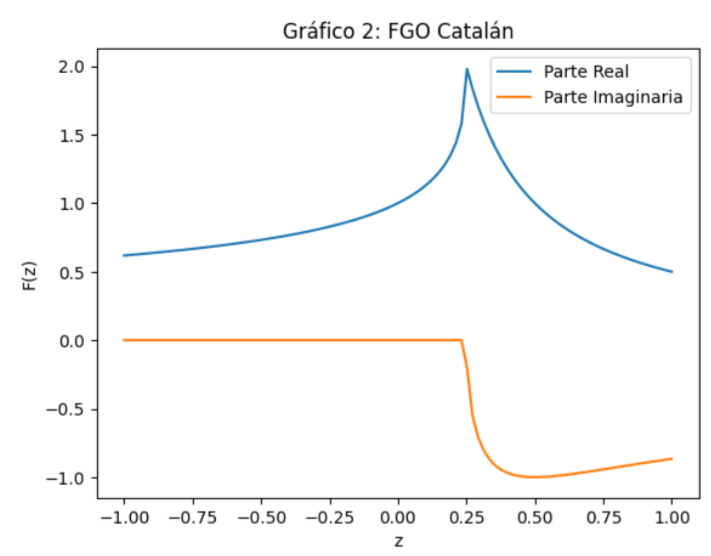
\includegraphics[width= 90 mm]{imagenes-gráficas/fgo_2.png}
    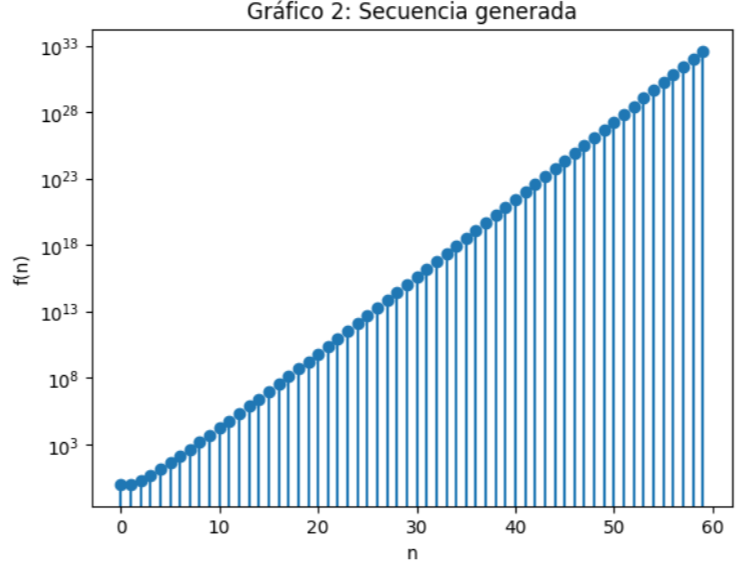
\includegraphics[width= 90 mm]{imagenes-gráficas/secuencia_2.png}
         
    \item\,[*] $f(n)=\left\langle\dfrac{1}{2}, -1,-\dfrac{3}{2},-2,-2, 0,8,32,96,256,640,1536,\cdots\right\rangle_{n\ge 0}$\\
        No se realizó.
    \item\,[*]  $f(n)=\left\langle \sum_{0\leq k\leq n}{k\cdot (-1)^n\cdot (-1)^k}\right\rangle_{n\geq3}$ \\
    
\includegraphics[width= 10 mm]{figures/exc.png}(Estudiantes: Mariana Guerrero- 200173479 y Alejandra Landinez Lamadrid - 200161946)
    \cite{ChatGPT_sec}
    \begin{itemize}
        \item Versión recurrente: K es una variable: Si es par, k es divisible por 2, luego,  $(-1)^k = 1$. Si es impar, luego $(-1)^k =-1$ \\
            Es posible dividir la sumatoria para k par e impar\\
            
            Para k par, $k=2i$ para algún número entero i:
            
            $$\sum_{0\leq k\leq n} {k\cdot (-1)^n\cdot (-1)^k} = 2\sum_{0\leq i\leq n/2}{i}$$
            
            Para $k$ impar, $k = 2i+1$ para algún número entero i:
            
            $$\sum_{0\leq k\leq n} {k\cdot (-1)^n\cdot (-1)^k} = -\sum_{0\leq i\leq (n-1)/2}{(2i+1)}$$
            
            $$f(n) = 2\sum_{0\leq i\leq n/2}{i} - \sum_{0\leq i\leq (n-1)/2}{(2i+1)}$$
            
            $f(n)= \frac{n(n+3)}{4}$:
    
    \item FGO: $F(z) = \sum_{n\geq0} f(n) \cdot z^n$\\
        $F(z) = \sum_{n\geq0} \left(\frac{n(n+3)}{4}\right) \cdot z^n$\\
        $F(z) = \frac{1}{4} \sum_{n\geq0} n(n+3) z^n $\\
        División en dos partes:\\
        $F(z)= \frac{1}{4} \left(\sum_{n\geq0} n^2 \cdot z^n + 3\sum_{n\geq0} n \dot z^n\right)$\\
        Se encuentran la seria de potencias para n: \\ $\sum_{n\geq0} n^2 z^n = zF''(z)$ y $\sum_{n\geq0} n z^n = zF'(z)$ respectivamente\\
        La FGO es $F(z)= \frac{1}{4}\left(z\left(zF''(z) + 2zF'(z) + \frac{1}{1-z}\right) + 3zF'(z)\right)$
    \end{itemize}
    Gráficas FGO y f(n)\\
    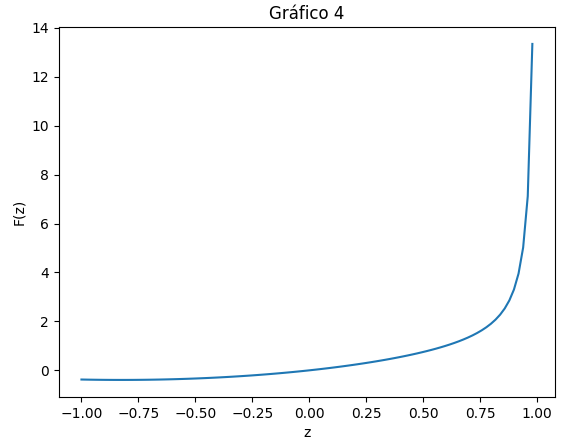
\includegraphics[width= 90 mm]{imagenes-gráficas/fgo_4.png}
    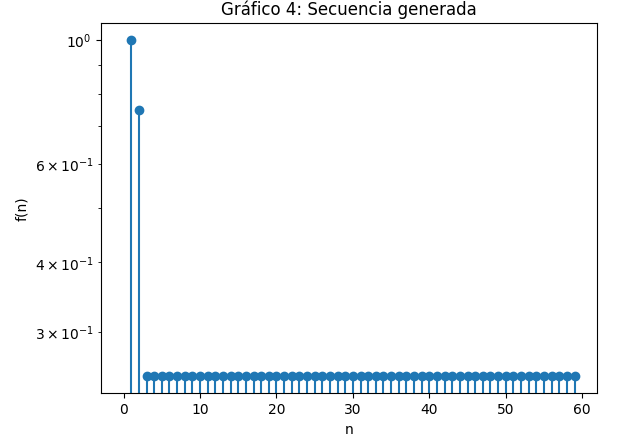
\includegraphics[width= 90 mm]{imagenes-gráficas/secuencias_4.png}
    
    \item $f_n=(n-1)(f_{n-1}+f_{n-2}), \quad f_1=0,\quad f_2=1,\quad n> 2.$\\
        \vspace{2 mm}
        
\includegraphics[width= 10 mm]{figures/exc.png}(Estudiante Mariana Guerrero- 200173479)\\
        $f_n = (n-1)f_{n-1}+(n-1)f_{n-2}$\\
        $f_n = (n-1)f_{n-1}+(n-2+1)f_{n-2}$\\
        $f(n) = (n-1)f(n-1)+(n-2)f(n-2)+ f(n-2)$\\
        $\sum_{n\geq3}f_n \cdot z^n = \sum_{n\geq3}(n-1)f_{n-1} \cdot z^n + \sum_{n\geq3}(n-2)f_{n-2} \cdot z^n + \sum_{n\geq3} f_{n-2} \cdot z^n$\\
        $-(f_0\cdot z^0+f_1\cdot z^1-f_2 \cdot z^2)+\sum_{n\ge0}f_n\cdot z^n =z^2\sum_{n\ge0}(n+1)f_{n+1} \cdot z^n-z^2(1)f_1+z^3\sum_{n\ge0}(n+1)f_{n+1} \cdot z^n + z^2 \sum_{n\ge0} f_n \cdot z^n$\\ 
        $\sum_{n\ge0}f_n\cdot z^n - f_0z^0 - f_1z^1 + f_2z^2 = z^2 F'(z) + z^3 F'(z) + z^2 F(z) $\\
        $F(z) - z^2 = z^2  F'(z) + z^3  F'(z) + z^2 F(z)$\\
        Pasamos $F(z)$ para la izquierda\\
        $F(z)-z^2F(z)= z^2  F'(z) + z^3  F'(z) + z^2 $\\
        $(1-z^2)F(z)= z^2  F'(z) + z^3  F'(z) + z^2 $\\
        Despejamos $F(z)$\\
        $F(z)= \dfrac{z^2 F'(z) + z^3 F'(z) + z^2}{(1-z^2)}$\\
    Gráficas FGO y f(n)\\
    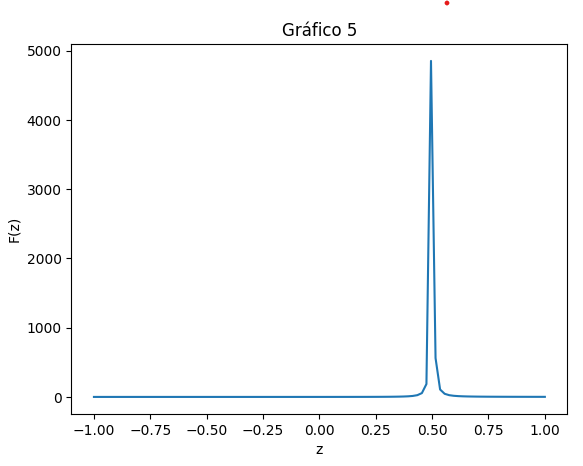
\includegraphics[width= 90 mm]{imagenes-gráficas/fgo_5.png}
    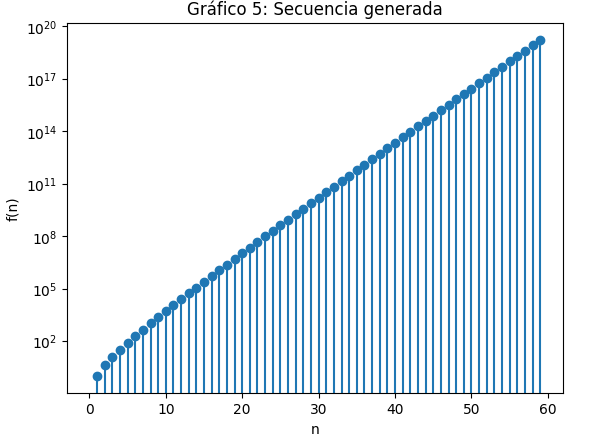
\includegraphics[width= 90 mm]{imagenes-gráficas/secuencias_5.png}

    Para cada una de las siguientes funciones generadoras ordinarias, encuentre una fórmula cerrada para la secuencia que esta determina.
    \item \,[*] $F(z) = \dfrac{z}{1-4z+4z^2}$
    \\
    
\includegraphics[width= 10 mm]{figures/exc.png}(Estudiantes: Alejandra Landinez Lamadrid - 200161946)
    \\
    \begin{align*}
        F(z) &= \frac{z}{1-4z+4z^2}\\
        &= \frac{z}{4z^2-4z+1}\\
        &= \frac{z}{(2z-1)^2}\\ 
    \end{align*}
    Usando fracciones parciales:
    \begin{align*}
        F(z) &= \frac{A}{2z-1} + \frac{B}{(2z-1)^2}\\
        z &= \frac{A}{2z-1}\cdot(2z-1)^2 + \frac{B}{(2z-1)^2} \cdot(2z-1)^2\\
        &= A(2z-1) + B(1)\\
        &= A(2z-1) + B
    \end{align*}
    \\
    \\
    Calculamos A:\\
        $z = A(2z-1)\\
        A = \frac{-z}{2z-1}$\\
    Calculamos B en $z = 0$:\\
    $z = B\\
    B = 0$\\
    Reemplazando los valores en F(Z):\\
    \begin{align*}
        F(z) &= \frac{-z}{2z-1} + 0\\
        &= -z\cdot \sum_{n\geq0} (2z)^n\\
        &= -\sum_{n\geq0} 2^{n+1}\cdot z^{n+1}\\
        &= -\sum_{n\geq1} 2^n \cdot z^n
    \end{align*}\\
    $f(n) &= -2^n, n\geq1$\\
    Gráficas FGO y f(n)\\
    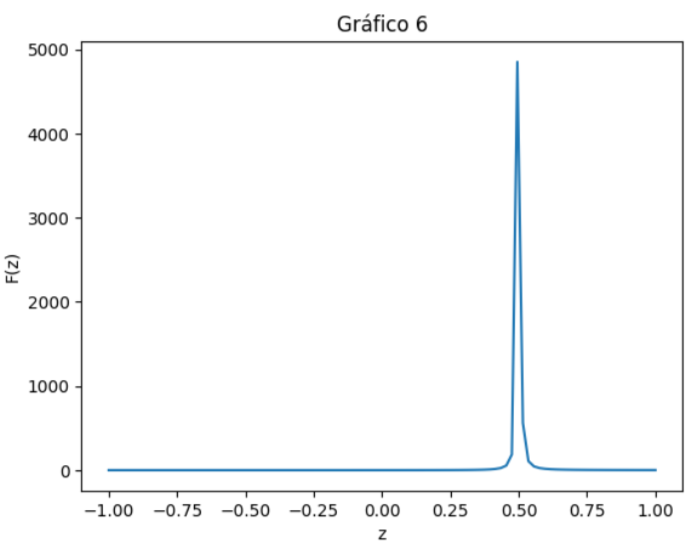
\includegraphics[width= 90 mm]{imagenes-gráficas/fgo_6.png}
    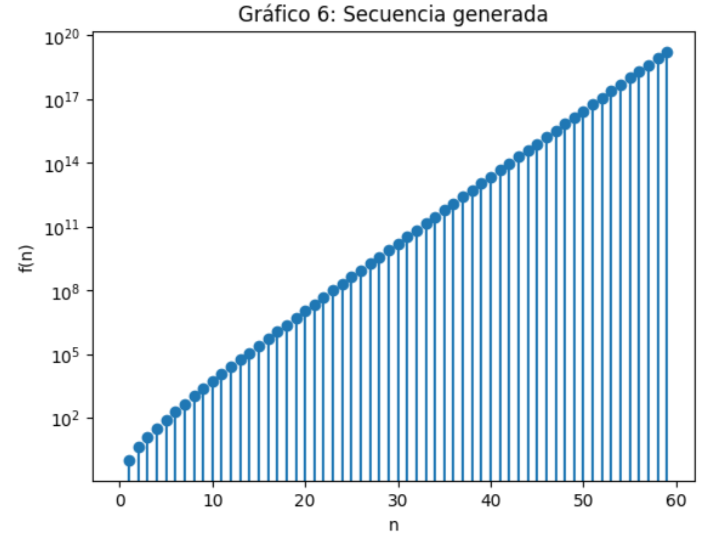
\includegraphics[width= 90 mm]{imagenes-gráficas/secuencias_6.png}

    \item \,[*] $F(z) = \dfrac{z}{1-3z-z^2+3z^3}$\\
    
\includegraphics[width= 10 mm]{figures/exc.png}(Estudiante: Alejandra Landinez Lamadrid - 200161946)\\
    \begin{align*}
        F(z) &= \frac{z}{1-3z-z^2+3z^3}\\
        &= \frac{z}{3z^3-z^2-3z+1}\\
        &= \frac{z}{(z-1)(3z^2+2z-1)}\\
        &= \frac{z}{(z-1)(z+1)(3z-1)}
    \end{align*}\\
    Usando fracciones parciales:\\
    \begin{align*}
        F(z) &= \frac{A}{z-1} + \frac{B}{z+1} + \frac{C}{3z-1}\\
        z &= A(3z^2+2z-1 + B(z-1)(z+1) + C(z-1)(3z-1)
    \end{align*}\\\
    z = 1\\
    \begin{align*}
        1 &= A(2)(2) + B(0)(2) + C(0)(2)\\
        1 &= 4A\\
        A &= \frac{1}{4}
    \end{align*}\\
    z = -1\\
    \begin{align*}
        -1 &= A(-4)(0) + B(-2)(0) + C(-2)(-4)\\
        -1 &= -8C\\
        C &= \frac{1}{8}
    \end{align*}\\
    z = 0\\
    \begin{align*}
        0 &= A(3(0)-1)(0+1) + B(0-1)(0+1) + C(0-1)(3(0)-1)\\
        0 &= -A-B+C\\
        0 &= \frac{-1}{4} - B +\frac{1}{8}\\
        \frac{1}{4} - \frac{1}{8} &= -B\\
        B &= \frac{-1}{4} + \frac{1}{8}\\
        B &= -\frac{1}{8}
    \end{align*}\\
    Reemplazamos en la ecuación original:\\
    \begin{align*}
        F(z) &= \frac{1}{4} \cdot \frac{1}{z-1} -\frac{1}{8} \cdot \frac{1}{z+1} + \frac{1}{8} \cdot \frac{1}{3z-1}\\
        &= -\frac{1}{4} \cdot\sum_{n\geq0} z^n -\frac{1}{8} \cdot\sum_{n\geq0} (-1)^n z^n + \frac{1}{24} \cdot\sum_{n\geq0} \left(\frac{1}{3}\right)^n\\
        &= \sum_{n\geq0} z^n \left(-\frac{1}{4}-\frac{1}{8} \cdot(-1)^n +\frac{1}{24} \left(\frac{1}{3}\right)^n\right)\\
        f(n) &= -\frac{1}{4} -\frac{1}{8} \cdot(-1)^n +\frac{1}{24} \cdot\left(\frac{1}{3}\right)^n
    \end{align*}
    Gráficas FGO y f(n)\\
    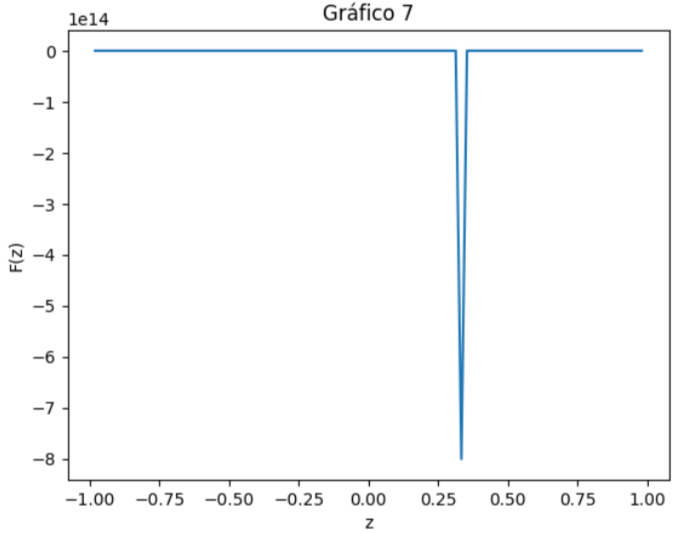
\includegraphics[width= 90 mm]{imagenes-gráficas/fgo_7.png}
    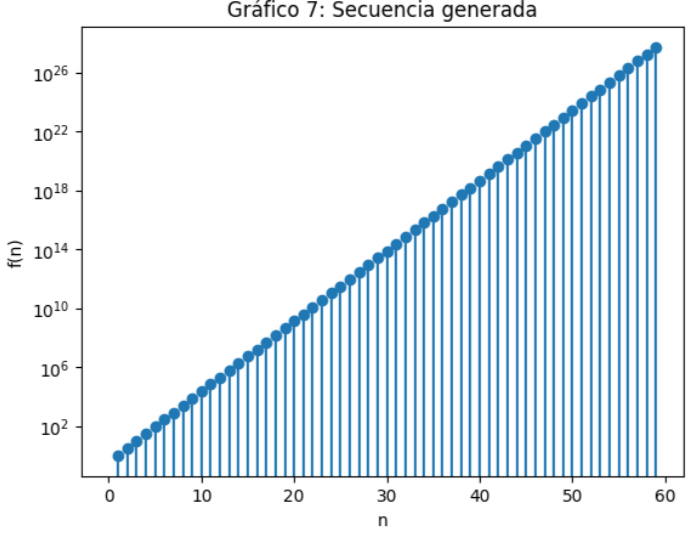
\includegraphics[width= 90 mm]{imagenes-gráficas/secuencias_7.png}

    \item \,[*] $F(z) - z + 1 = 9\cdot z\cdot (F(z)+1)-20\cdot z^2\cdot F(z)$\\
    \begin{align*}
        F(z) - z + 1 &= 9\cdot z\cdot (F(z)+1)-20\cdot z^2\cdot F(z)\\
        F(z) - 9\cdot z\cdot (F(z)-1) + 20\cdot z^2 \cdot F(z) &= z-1\\
        F(z) -9zF(z) - 9z + 20\cdot z^2 \cdot F(z) &= z-1\\
        F(z)\cdot (1 - 9z +20z^2) &= z-1+9z\\ 
        F(z)\cdot (1 - 9z +20z^2) &= 10z -1\\
        F(z) &= \frac{10z-1}{(1-5z)(1-4z)}\\
    \end{align*}\\
    Usando fracciones parciales:\\
    \begin{align*}
        F(z) &= \frac{A}{1-5z} +\frac{B}{1-4z}\\
        10z-1 &= A(1-4z) + B(1-5z)\\
        10z-1 &= A - 4Az + B - 5Bz\\
        10z-1 &= (A+B) + z(-4A - 5B)\\
        \frac{10z-1}{z} &= A + B -4A -5B\\
    \end{align*}
    Gráficas FGO y f(n)\\
    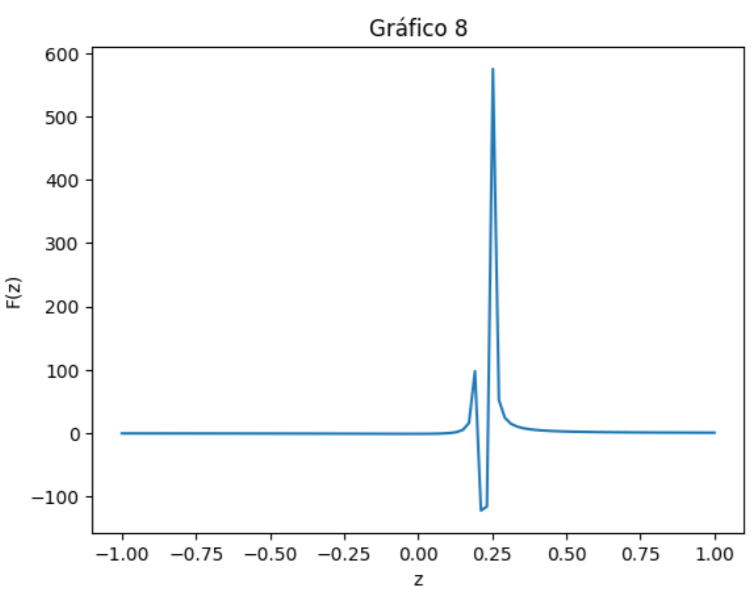
\includegraphics[width= 90 mm]{imagenes-gráficas/fgo_8.png}
    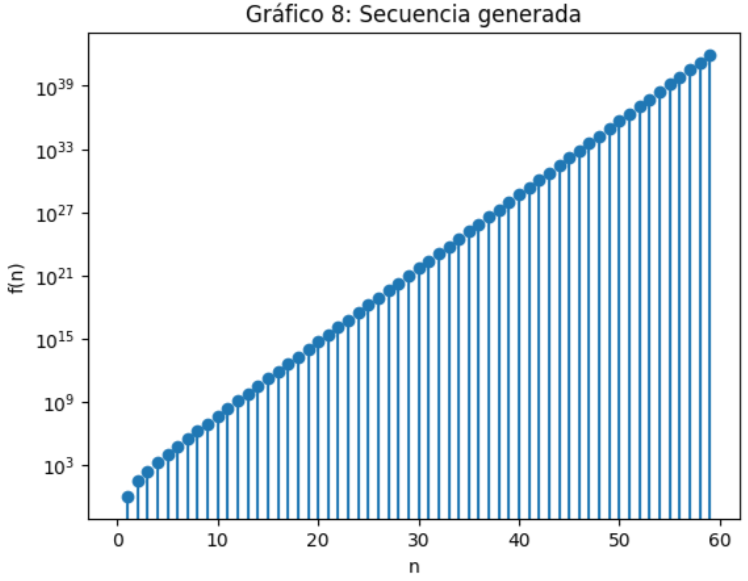
\includegraphics[width= 90 mm]{imagenes-gráficas/secuencias_8.png}
\end{enumerate}
%

%***********************

\section*{Problema 2: Ejercicios para codificar en python. PC-ED-El Man-202330.ipynb}
\href{https://colab.research.google.com/drive/1vCZkVY7bXAuF_cyLY6kDvWL_nf0ut6MD?usp=sharing#scrollTo=a_GFcCmwZ7k7}{\textcolor{blue}{\underline{Código Python en Colab}}}
\begin{enumerate}
\item \,[*] Tensores \\ Diseñe e implemente cinco emoji logo
\begin{itemize}
    \item Uninorte (Estudiante Juan Camilo Aguirre - 200156480)
    \begin{center}
    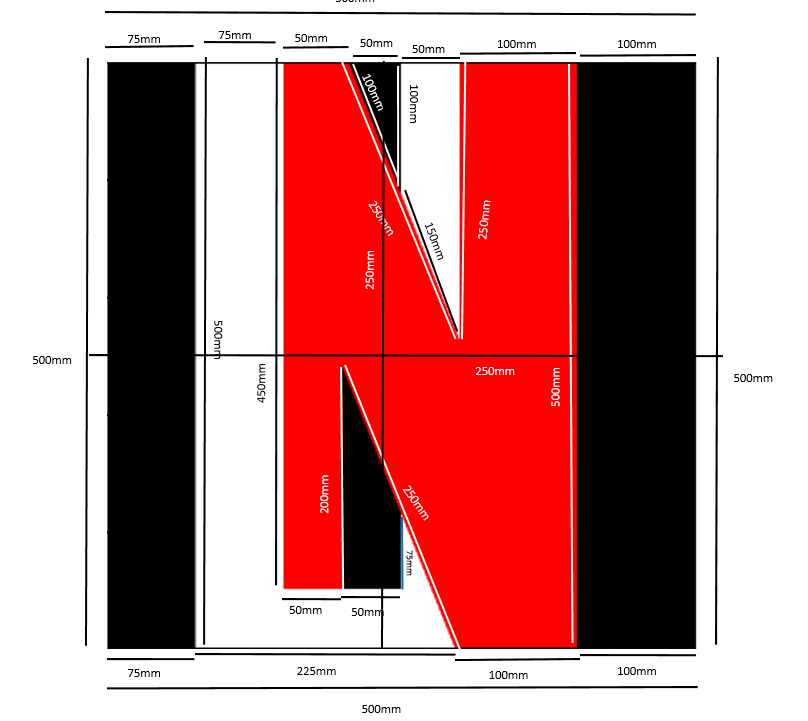
\includegraphics[width=125mm]{imagenes-colab/maquetaun.png}
    \end{center}
    \begin{lstlisting}[language=Python]
    import cv2
    import numpy as np
    import matplotlib.pyplot as plt
    from google.colab.patches import cv2_imshow
    
    imagen = np.zeros((500, 500, 3), dtype=np.uint8)
    imagen.fill(0)
    plt.imshow(imagen)
    
    imagen[:,:,:]=(0,0,0)
    
    imagen[:,100:200,:]=(255,0,0)
    imagen[:,300:400,:]=(255,0,0)
    
    imagen[:,250:300,:]=(255,255,255)
    imagen[:,100:150,:]=(255,255,255)
    imagen[450:500,100:300,:]=(255,255,255)
    
    color = (255, 0, 0)
    grosor= 100
    puntoUN1 = (150, 0)
    puntoUN2 = (350, 500)
    cv2.line(imagen, puntoUN1, puntoUN2, color, grosor)
    imagen[:,75:150,:]=(255,255,255)
    
    plt.imshow(imagen)
    print("La U es blanca y la N es roja")
    \end{lstlisting}
    
    \item División de Ingenierías  (Estudiante Juan Camilo Aguirre - 200156480)
    \begin{center}
    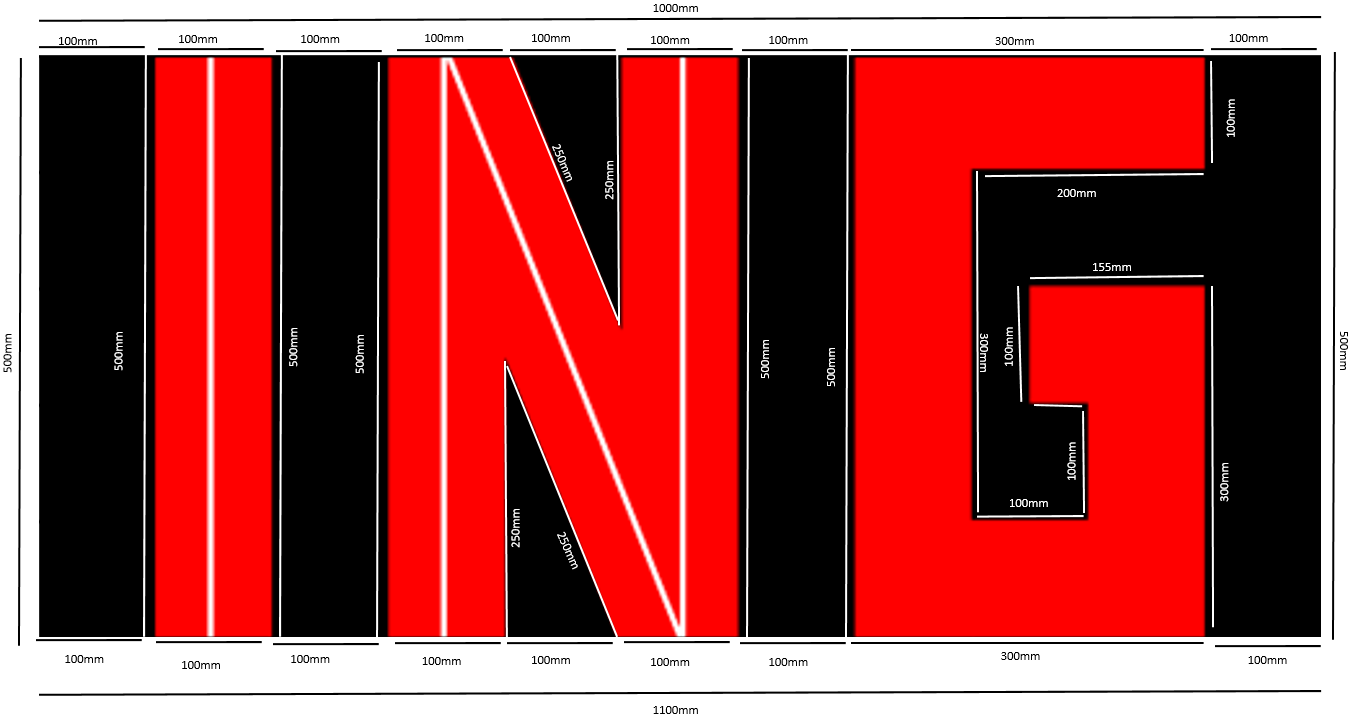
\includegraphics[width=125mm]{imagenes-colab/maquetaing.png}
    \end{center}
    \begin{lstlisting}[language=Python]
    #Division de Ingenierias
    import cv2
    import numpy as np
    import matplotlib.pyplot as plt
    
    from google.colab.patches import cv2_imshow
    
    imagen = np.zeros((500,1100, 3), dtype=np.uint8)
    imagen.fill(255)
    plt.imshow(imagen)
    color_linea = (255, 0, 0)
    grosor_linea = 100
    
    imagen[:,:,:]=(0,0,0)
    
    imagen[:,100:200,:]=(255,0,0)
    
    imagen[:,300:400,:]=(255,0,0)
    puntoING1=(350,0)
    puntoING2=(550,500)
    imagen[:,500:600,:]=(255,0,0)
    cv2.line(imagen,puntoING1,puntoING2,color_linea,grosor_linea)
    
    
    imagen[0:100,700:900,:]=(255,0,0)
    
    imagen[400:500,750:1000,:]=(255,0,0)
    imagen[0:100,750:1000,:]=(255,0,0)
    
    imagen[:,700:800,:]=(255,0,0)
    
    imagen[200:500,900:1000,:]=(255,0,0)
    
    imagen[200:300,850:900,:]=(255,0,0)
    
    imagen[:,145:150,:]=(255,255,255)
    imagen[:,145:150,:]=(255,255,255)
    
    imagen[:,345:350,:]=(255,255,255)
    
    imagen[:,550:555,:]=(255,255,255)
    
    puntoING3=(350,0)
    puntoING4=(550,500)
    color = (255, 255, 255)
    grosor = 3
    cv2.line(imagen,puntoING3,puntoING4,color,grosor)
    
    plt.imshow(imagen)
    \end{lstlisting}
    \item Departamento de Ingeniería de Sistemas (Estudiante Juan Camilo Aguirre - 200156480)
    \begin{center}
    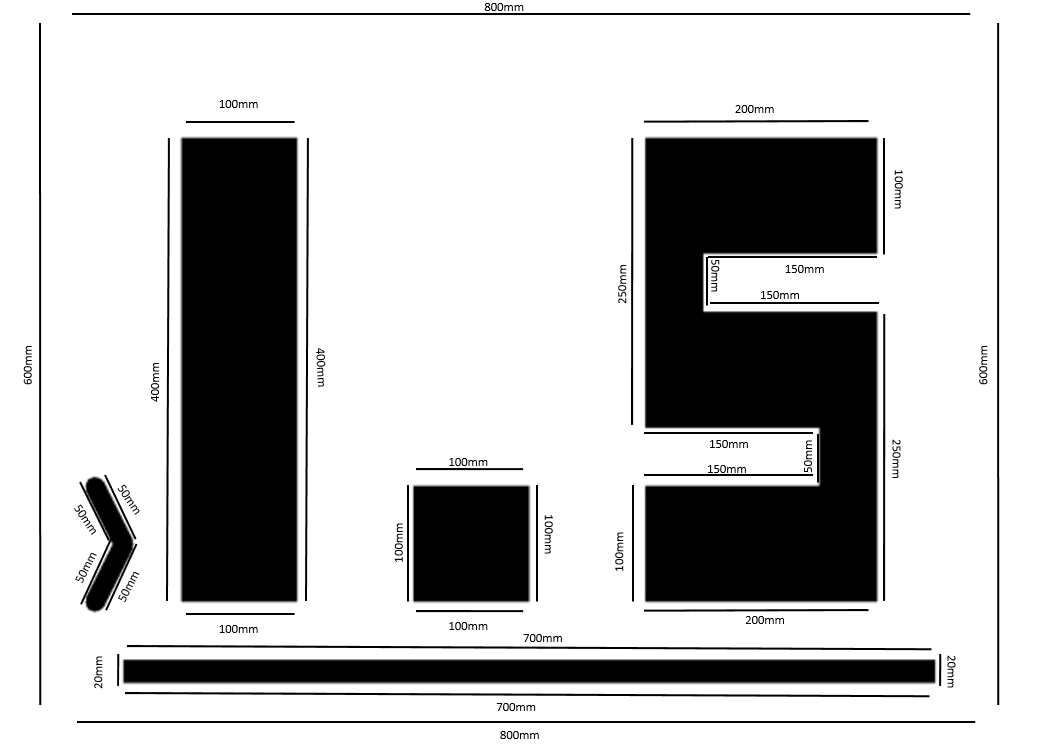
\includegraphics[width=125mm]{imagenes-colab/maquetais.png}
    \end{center}
    \begin{lstlisting}[language=Python]
    #Logo del departamento de Ingenieria de Sistemas

    import cv2
    import numpy as np
    import matplotlib.pyplot as plt
    
    imagen = np.zeros((600,800, 3), dtype=np.uint8)
    imagen.fill(255)
    plt.imshow(imagen)
    
    imagen[100:500,100:200,:]=(0,0,0)
    imagen[400:500,300:400,:]=(0,0,0)
    imagen[400:500,500:700,:]=(0,0,0)
    imagen[100:200,500:700,:]=(0,0,0)
    imagen[200:300,500:550,:]=(0,0,0)
    imagen[200:300,500:550,:]=(0,0,0)
    imagen[250:350,500:700,:]=(0,0,0)
    imagen[300:400,650:700,:]=(0,0,0)
    imagen[550:570,50:750,:]=(0,0,0)
    
    puntoIS1=(25,400)
    puntoIS2=(25,500)
    puntoIS3=(50,450)
    color=(0,0,0)
    grosor=15
    
    cv2.line(imagen,puntoIS1,puntoIS3,color,grosor)
    cv2.line(imagen,puntoIS2,puntoIS3,color,grosor)
    
    plt.imshow(imagen)
    \end{lstlisting}
    \item Cruz roja internacional (Estudiante Mariana Guerrero Benavides-200173479)
    \begin{center}
    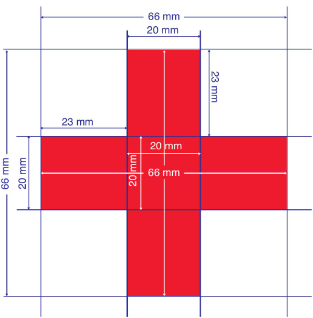
\includegraphics[]{figures/Logo cruz roja.png}
    \end{center}
    \begin{lstlisting}[language=Python]
    import numpy as np
    import matplotlib.pyplot as plt
    
    # medidas estandar del logo Cruz Roja (en mm)
    ancho = 66  ; alto = 66
    # espesor del brazo de la cruz (20mm)
    b = int(ancho / 3)
    # espacio alrededor de la cruz(6 mm)
    margen = 3
    # area total del gráfico
    ancho_total = ancho + 2 * margen ; alto_total = alto + 2 * margen
    # tensor con pixeles blancos
    cruz_roja = np.ones((alto_total, ancho_total, 3), dtype=np.uint8)* 255
    cruz_roja=cruz_roja[:,:,::-1]
    rojo = (255, 0, 0)
    # fila central
    fila = alto_total // 2
    cruz_roja[fila - b // 2 : fila + b // 2, margen : ancho_total - margen, :] = rojo
    # columna central
    columna = ancho_total // 2
    cruz_roja[margen : alto_total - margen, columna - b // 2 : columna + b // 2, :] = rojo
    plt.imshow(cruz_roja)
    plt.show()
    \end{lstlisting}
    \item Excelente  (Estudiante Juan Camilo Aguirre - 200156480)
    \begin{center}
    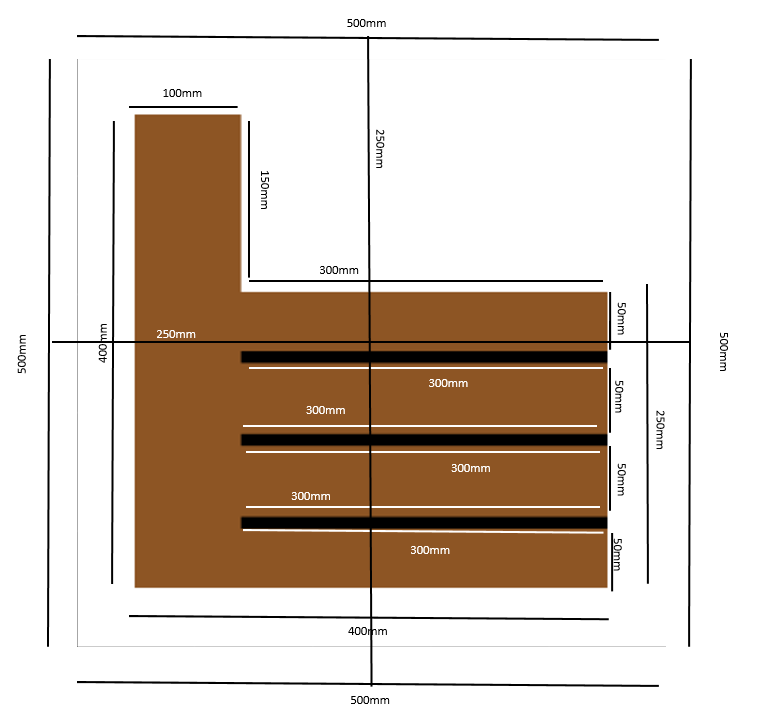
\includegraphics[width=125mm]{imagenes-colab/maquetaex.png}
    \end{center}
    \begin{lstlisting}[language=Python]
    #Excelente
    import cv2
    import numpy as np
    from google.colab.patches import cv2_imshow
    
    imagen = np.zeros((500, 500, 3), dtype=np.uint8)
    imagen.fill(255)
    plt.imshow(imagen)
    
    imagen[200:450, :, :]=[141,85,36] #piel
    imagen[:,50:140,:]=[141,85,36] #piel
    imagen[450:500, :, :]=[255,255,255] #blanco
    imagen[0:50, :, :]=[255,255,255] #blanco
    imagen[:,0:50,:]=[255,255,255] #blanco
    imagen[:,450:500,:]=[255,255,255] #blanco
    imagen[250:260, :, :]=[0,0,0] #linea negra
    imagen[320:330, :, :]=[0,0,0] #linea negra
    imagen[390:400, :, :]=[0,0,0] #linea negra
    imagen[:,0:50,:]=[255,255,255] #blanco
    imagen[:,450:500,:]=[255,255,255] #blanco
    imagen[:,50:140,:]=[141,85,36] #piel
    imagen[450:500, :, :]=[255,255,255] #blanco
    imagen[0:50, :, :]=[255,255,255] #blanco
    
    plt.imshow(imagen)
    \end{lstlisting}
\end{itemize}
Anexe la plantilla correspondiente, con las dimensiones establecidas 


\includegraphics[width= 10 mm]{figures/exc.png} (Mariana Guerrero Benavides y Juan Camilo Aguirre (200173479 y 200156480 respectivamente))

    \item \,[*] Imprima el triángulo de $Bell$ y las particiones correspondientes para $0\le n < 10$. Ejemplo, para $B(3)=5$ las particiones son: 
    \begin{itemize}
        \item $\{\; \{1\}\cup \{2\}\cup \{3\}\; \}$
        \item $\{\; \{1, 2\}\cup \{3\} \;\} $
        \item $\{\; \{1, 3\}\cup \{2\}\; \}$
        \item $\{\; \{2, 3\}\cup \{1\}\; \}$
        \item $ \{1, 2, 3\} $

    \end{itemize}

    \cite{ChatGPT_Bell}
    
    
\includegraphics[width= 10 mm]{figures/exc.png} (Estudiante Mariana Guerrero Benavides-200173479)
    \begin{lstlisting} [language=Python]
def triangulo_bell(n):
    # inicializamos el triangulo con B(0) = 1
    triangulo = [[0] * (n + 1) for _ in range(n + 1)]
    triangulo[0][0] = 1

    # calculamos el triangulo de Bell utilizando recurrencia
    for i in range(1, n + 1):
        triangulo[i][0] = triangulo[i - 1][i - 1]
        for j in range(1, i + 1):
            triangulo[i][j] = triangulo[i - 1][j - 1] + triangulo[i][j - 1]
    return triangulo

def particiones_conj(n):
    # se calcula el triangulo de bell
    triangulo = triangulo_bell(n)
    
    # generamos particiones correspondientes para 0 <= n < 10
    particiones = []
    for k in range(1, n + 1):
        particion_k = []
        for i in range(n + 1):
            if triangulo[i][k] != 0:
                particion_k.append(set(range(i - k + 1, i + 1)))
        particiones.append(particion_k)
    return particiones
       
# imprimimos el triangulo de bell
print(f"Triangulo de Bell para 0 <= n < 10:")
for row in triangulo_bell(9):
    row_values = [str(value) for value in row if value != 0]
    print(" ".join(row_values))
print()
# imprimimos particiones correspondientes para 0 <= n < 10
for n in range(10):
    valor = triangulo_bell(n)[n][0]
    particiones = particiones_conj(n)
    print(f"B({n}) = {valor}, las particiones correspondientes son:")
    for i, particion in enumerate(particiones):
        print(f"- {particion}")
print()
    \end{lstlisting}
    \item \,[*] Gráficas de las secuencias y FGO de todos los ejercicios de Funciones Generadoras y Secuencias..\\
    Entrada: $F(z), -1 < z < 1$ y $ f(n),\, n>=0$ \\
    Salida: Las gráficas correspondientes

    \cite{secuencia_FGO}
    
    (Estudiante Mariana Guerrero Benavides-200173479)
    \begin{lstlisting}[language=Python]
    from numbers import Real
import numpy as np
import sympy as sp
import matplotlib.pyplot as plt
from IPython.display import display, Math

z = sp.symbols('z') # definimos z como una variable simbólica

# valores de z en intervalo (-1, 1)
Z = np.linspace(-1, 1, 100)


# definimos las FGO
def fgo_1(z):
    return 1 / (1 - z- z**2) 

def fgo_2(z):
    return (1 - (sp.sqrt(1-4*z)))/(2*z)  
'''
def fgo_3(z):
    return
'''
def fgo_4(z):
  Fz = z # ajustar segun necesidad
  F_doble_prima = Fz.diff(z, 2) # derivada de Fz
  F_prima = Fz.diff(z) # segunda derivada de Fz

  return (1/4) * (z * (z * F_doble_prima + 2 * z * F_prima + 1 / (1 - z)) + 3 * z * F_prima)

def fgo_5(z):
    return z / (1 - 4 * z + 4 * z**2)

def fgo_6(z):
  return z/(1-4*z+ 4*z**2)

def fgo_7(z):
  return z/(1-3*z-z**2+3*z**3)

def fgo_8(z):
  return ((10*z-1)/((1-5*z)*(1-4*z)))


n=60
# Crea y muestra el gráfico primer FGO
plt.plot(Z, [fgo_1(z) for z in Z])
plt.title('Gráfico 1: FGO')
plt.xlabel('z') , plt.ylabel('F(z)')
plt.show()
display(Math(sp.latex(fgo_1(z)))) # imprimimos la FGO en Látex
# calculamos la secuencia generada a partir de la FGO
Fz_1 = sp.Poly(fgo_1(z).series(x=z, x0=0,n=n).removeO())
fn_1=Fz_1.all_coeffs()
print('Secuencia generada\n',fn_1[::-1]) # imprimimos la secuencia generada
# rango de valores de n
n_1 = np.arange(len(fn_1))
plt.yscale('log')  # Cambia la escala a logarítmica en el eje y
# Crea y muestra gráfico de la secuencia generada
plt.stem(n_1, fn_1[::-1])
plt.xlabel('n') , plt.ylabel('f(n)')
plt.title('Gráfico 1: Secuencia generada')
plt.show()

# Crea y muestra el gráfico segunda FGO
# Calcula la función fgo_2 para los valores de Z
valores = [fgo_2(z_val) for z_val in Z]
# Separa las partes real e imaginaria de los resultados
real = [sp.re(val) for val in valores]
imaginario = [sp.im(val) for val in valores]
# Crea y muestra el gráfico de la parte real e imaginaria
plt.plot(Z, real, label='Parte Real'), plt.plot(Z, imaginario, label='Parte Imaginaria')
plt.title('Gráfico 2: FGO Catalán')
plt.xlabel('z'), plt.ylabel('F(z)')
plt.legend(), plt.show()
display(Math("FGO: "+ sp.latex(fgo_2(z)))) # imprimimos la FGO en Látex
# calculamos la secuencia generada a partir de la FGO
Fz_2 = sp.Poly(fgo_2(z).series(x=z, x0=0,n=n).removeO())
fn_2=Fz_2.all_coeffs()
print('Secuencia generada\n',fn_2[::-1]) # imprimimos la secuencia generada
# rango de valores de n
n_2 = np.arange(len(fn_2))
plt.yscale('log')  # Cambia la escala a logarítmica en el eje y
# Crea y muestra gráfico de la secuencia generada
plt.stem(n_2, fn_2[::-1])
plt.xlabel('n') , plt.ylabel('f(n)')
plt.title('Gráfico 2: Secuencia generada')
plt.show()
'''
# Crea y muestra el gráfico tercera FGO
plt.plot(Z, [fgo_3(z) for z in Z])
plt.title('Gráfico 3')
plt.xlabel('z') , plt.ylabel('F(z)')
plt.show()
display(Math("FGO: "+ sp.latex(fgo_3(z)))) # imprimimos la FGO en Látex
# calculamos la secuencia generada a partir de la FGO
Fz_3 = sp.Poly(fgo_3(z).series(x=z, x0=0,n=n).removeO())
fn_3=Fz_3.all_coeffs()
print('Secuencia generada\n',fn_3[::-1]) # imprimimos la secuencia generada
# rango de valores de n
n_3 = np.arange(len(fn_3))
plt.yscale('log')  # Cambia la escala a logarítmica en el eje y
# Crea y muestra gráfico de la secuencia generada
plt.stem(n_3, fn_3[::-1])
plt.xlabel('n') , plt.ylabel('f(n)')
plt.title('Gráfico 3: Secuencia generada')
plt.show()
'''
# Crea y muestra el gráfico cuarta  FGO
fun_num1 = sp.lambdify(z, fgo_4(z), 'numpy') # convertimos la función en una función numérica
val_func1 = fun_num1(Z)
plt.plot(Z, val_func1)
plt.title('Gráfico 4')
plt.xlabel('z') , plt.ylabel('F(z)')
plt.show()
display(Math("FGO: "+ sp.latex(fgo_4(z)))) # imprimimos la FGO en Látex
# calculamos la secuencia generada a partir de la FGO
Fz_4 = sp.Poly(fgo_4(z).series(x=z, x0=0,n=n).removeO())
fn_4=Fz_4.all_coeffs()
print('Secuencia generada\n',fn_4[::-1]) # imprimimos la secuencia generada
# rango de valores de n
n_4 = np.arange(len(fn_4))
plt.yscale('log')  # Cambia la escala a logarítmica en el eje y
# Crea y muestra gráfico de la secuencia generada
plt.stem(n_4, fn_4[::-1])
plt.xlabel('n') , plt.ylabel('f(n)')
plt.title('Gráfico 4: Secuencia generada')
plt.show()


# Crea y muestra el gráfico quinta FGO
plt.plot(Z, [fgo_5(z) for z in Z])
plt.title('Gráfico 5')
plt.xlabel('z') , plt.ylabel('F(z)')
plt.show()
display(Math("FGO: "+sp.latex(fgo_5(z)))) # imprimimos la FGO en Látex
# calculamos la secuencia generada a partir de la FGO
Fz_5 = sp.Poly(fgo_5(z).series(x=z, x0=0,n=n).removeO())
fn_5=Fz_5.all_coeffs()
print('Secuencia generada\n',fn_5[::-1]) # imprimimos la secuencia generada
# rango de valores de n
n_5 = np.arange(len(fn_5))
plt.yscale('log')  # Cambia la escala a logarítmica en el eje y
# Crea y muestra gráfico de la secuencia generada
plt.stem(n_5, fn_5[::-1])
plt.xlabel('n') , plt.ylabel('f(n)')
plt.title('Gráfico 5: Secuencia generada')
plt.show()

# Crea y muestra el gráfico sexta FGO
plt.plot(Z, [fgo_6(z) for z in Z])
plt.title('Gráfico 6')
plt.xlabel('z') , plt.ylabel('F(z)')
plt.show()
display(Math("FGO: "+sp.latex(fgo_6(z)))) # imprimimos la FGO en Látex
# calculamos la secuencia generada a partir de la FGO
Fz_6 = sp.Poly(fgo_6(z).series(x=z, x0=0,n=n).removeO())
fn_6=Fz_6.all_coeffs()
print('Secuencia generada\n',fn_6[::-1]) # imprimimos la secuencia generada
# rango de valores de n
n_6 = np.arange(len(fn_6))
plt.yscale('log')  # Cambia la escala a logarítmica en el eje y
# Crea y muestra gráfico de la secuencia generada
plt.stem(n_6, fn_6[::-1])
plt.xlabel('n') , plt.ylabel('f(n)')
plt.title('Gráfico 6: Secuencia generada')
plt.show()

# Crea y muestra el gráfico septima FGO
plt.plot(Z, [fgo_7(z) for z in Z])
plt.title('Gráfico 7')
plt.xlabel('z') , plt.ylabel('F(z)')
plt.show()
display(Math("FGO: "+ sp.latex(fgo_7(z)))) # imprimimos la FGO en Látex
# calculamos la secuencia generada a partir de la FGO
Fz_7 = sp.Poly(fgo_7(z).series(x=z, x0=0,n=n).removeO())
fn_7=Fz_7.all_coeffs()
print('Secuencia generada\n',fn_7[::-1]) # imprimimos la secuencia generada
# rango de valores de n
n_7 = np.arange(len(fn_7))
plt.yscale('log')  # Cambia la escala a logarítmica en el eje y
# Crea y muestra gráfico de la secuencia generada
plt.stem(n_7, fn_7[::-1])
plt.xlabel('n') , plt.ylabel('f(n)')
plt.title('Gráfico 7: Secuencia generada')
plt.show()

# Crea y muestra el gráfico octava FGO
fun_num = sp.lambdify(z, fgo_8(z), 'numpy') # convertimos la función en una función numérica
val_func = fun_num(Z)
plt.plot(Z, val_func)
plt.title('Gráfico 8')
plt.xlabel('z') , plt.ylabel('F(z)')
plt.show()
display(Math("FGO: "+ sp.latex(fgo_8(z)))) # imprimimos la FGO en Látex
# calculamos la secuencia generada a partir de la FGO
Fz_8 = sp.Poly(fgo_8(z).series(x=z, x0=0,n=n).removeO())
fn_8=Fz_8.all_coeffs()
print('Secuencia generada\n',fn_8[::-1]) # imprimimos la secuencia generada
# rango de valores de n
n_8 = np.arange(len(fn_8))
plt.yscale('log')  # Cambia la escala a logarítmica en el eje y
# Crea y muestra gráfico de la secuencia generada
plt.stem(n_8, fn_8[::-1])
plt.xlabel('n') , plt.ylabel('f(n)')
plt.title('Gráfico 8: Secuencia generada')
plt.show()

    \end{lstlisting}
    \item \,[*] Gráficas 2D en coordenadas
    \begin{itemize}
        \item Cartesianas
        \item Polares
    \end{itemize} 
    Gráficas 3D en coordenadas
    \begin{itemize}
        \item Rectangulares
        \item Esféricas
        \item Cilíndricas
    \end{itemize}
    Diseñe los menus respectivos.\\
\textcolor{red}{Ayuda: utilice la siguiente referencia}
\href{https://www.uv.mx/personal/aherrera/files/2014/05/03-Sistemas-de-Coordenadas-en-3D-AHE.pdf}{\textcolor{blue}{\underline{Coordenadas en 3D}}}

\cite{ChatGPT_Graficas}


\includegraphics[width= 10 mm]{figures/exc.png}(Estudiante Mariana Guerrero Benavides-200173479)

\begin{lstlisting}[language=Python]
import matplotlib.pyplot as plt
from mpl_toolkits.mplot3d import Axes3D
import numpy as np

# Función que calcula f(x, y, z)
def funcion(x, y, z):
    return 3* np.sin(x) + 5* np.cos(y) + 2  # Cambiar la función según necesidades

def coord_cartesianas(funcion):
    # grillas de coordenadas
    x = np.linspace(-2*np.pi, 2*np.pi, 100)
    # evaluamos la función en cada valor de x
    y = []
    for val in x:
        y.append(funcion(val, 0, 0))

    plt.plot(x,y)
    plt.title('Coordenadas Cartesianas 2D')
    plt.xlabel('X'); plt.ylabel('Y')
    plt.show()

def coord_polares(funcion):
    # grillas de coordenadas
    theta = np.linspace(0, 2*np.pi, 100)
    # evaluamos la función en cada valor de theta
    r = []
    for val in theta:
      r.append(funcion(1, val, 0))
    
    plt.polar(theta, r)
    plt.title('Coordenadas Polares 2D')
    plt.show()

def coord_rectangulares(funcion):
    fig = plt.figure()
    ax = fig.add_subplot(111, projection='3d')
    # grillas de coordenadas
    x, y = np.linspace(-2, 2, 100), np.linspace(-2, 2, 100)
    X, Y = np.meshgrid(x, y)
    # evaluamos la función en x y y
    Z = []
    for x_row, y_row in zip(X, Y):
        row = []
        for x_val, y_val in zip(x_row, y_row):
            value = funcion(x_val, y_val, 0)
            row.append(value)
        Z.append(row)
    Z = np.array(Z)
    
    ax.plot_surface(X, Y, Z)
    plt.title('Coordenadas Rectangulares 3D')
    plt.show()

def coord_esfericas(funcion):
    fig = plt.figure()
    ax = fig.add_subplot(111, projection='3d')
    # grillas de coordenadas
    phi = np.linspace(0, 2*np.pi, 100)
    theta = np.linspace(0, np.pi, 100)
    PHI, THETA = np.meshgrid(phi, theta)
    # evaluamos la función en phi y theta
    R = []
    for phi_row, theta_row in zip(PHI, THETA):
        row = []
        for phi_val, theta_val in zip(phi_row, theta_row):
            value = funcion(1, theta_val, phi_val)
            row.append(value)
        R.append(row)
    R = np.array(R)
    # transformación coordenadas esféricas a rectangulares
    X = R * np.sin(THETA) * np.cos(PHI)
    Y = R * np.sin(THETA) * np.sin(PHI)
    Z = R * np.cos(THETA)

    ax.plot_surface(X, Y, Z)
    plt.title('Coordenadas Esféricas 3D')
    plt.show()

def coord_cilindricas(funcion):
    fig = plt.figure()
    ax = fig.add_subplot(111, projection='3d')
    # grillas de coordenadas
    theta = np.linspace(0, 2*np.pi, 100)
    z = np.linspace(-2, 2, 100)
    Theta, Z = np.meshgrid(theta, z)
    # evaluamos la función en theta y z
    R = []
    for theta_row, z_row in zip(Theta, Z):
        row = []
        for theta_val, z_val in zip(theta_row, z_row):
            value = funcion(1, theta_val, z_val)
            row.append(value)
        R.append(row)
    R = np.array(R)
    # transformación coordenadas cilíndricas a rectangulares
    X = R * np.cos(Theta)
    Y = R * np.sin(Theta)

    ax.plot_surface(X, Y, Z)
    plt.title('Coordenadas Cilíndricas 3D')
    plt.show()


# Menú principal
while True:
    print("** Menú principal **")
    print("Seleccione dimensión de la gráfica:")
    print("1. Coordenadas en 2D")
    print("2. Coordenadas en 3D")
    print("3. Salir")
    opcion = int(input("Escoja opción: "))
    print(" - - - - - - - - ")

    if opcion == 1:
      print("Coordenadas en 2D")
      while True:
        print("Seleccione el tipo de gráfica:")
        print("1. Coordenadas Cartesianas 2D")
        print("2. Coordenadas Polares 2D")
        print("3. Atras")
        print(" - - - - - - - - ")
        op = int(input("Escoja opción: "))
        if op == 1:
            coord_cartesianas(funcion)
        elif op == 2:
            coord_polares(funcion)
        elif op == 3:
          break
        else:
            print("Opción no válida. Por favor, ingrese una opción válida.")

    elif opcion == 2:
      print("Coordenadas en 3D")
      while True:
        print("Seleccione el tipo de gráfica:")
        print("1. Coordenadas Rectangulares 3D")
        print("2. Coordenadas Esféricas 3D")
        print("3. Coordenadas Cilíndricas 3D")
        print("4. Atras")
        print(" - - - - - - - - ")
        op = int(input("Escoja opción: "))
        if op == 1:
            coord_rectangulares(funcion)
        elif op == 2:
            coord_esfericas(funcion)
        elif op== 3:
            coord_cilindricas(funcion)
        elif op == 4:
            break
        else:
            print("Opción no válida. Por favor, ingrese una opción válida.")

    elif opcion == 3:
        print("Salida con éxito")
        break
    else:
        print("Opción no válida. Por favor, ingrese una opción válida.")
\end{lstlisting}
    \item \,[*] Solución de RRLNHCCC.\\
    Entrada: La expresión cerrada de la secuencia recurrente RRLNHCCC, $f(n)=f^H(n)+f^p(n)$, más condiciones iniciales. \\
    Salida: La expresión cerrada para secuencia NO recurrente $f(n)$ y los 25 primeros términos generados por ambas.\\
    
\includegraphics[width= 10 mm]{figures/exc.png}(Estudiante Mariana Guerrero Benavides-200173479)
    \begin{lstlisting}[language=Python]
    import sympy as sp

# Definimos variables simbólicas
n = sp.symbols('n')
x = sp.symbols('x')

# Definimos valor inicial
i0 = 1.0  # Ajustar según necesidades

# Encuentra raíces del polinomio
def calcular_raiz(coeficientes, i0):
  # Creamos el polinomio a partir de los coeficientes
  polinomio = sum(coef * x**i for i, coef in enumerate(coeficientes[::-1])) 
  raices = []
  for _ in range(len(coeficientes)):
    raiz = sp.solve(polinomio, x)
    if raiz:
      raices.append(raiz)
    coeficientes.pop(0)
    polinomio = sum(coef * x**i for i, coef in enumerate(coeficientes[::-1])) 
  return (raices)

# Encuentra la secuencia no recurrente
def calcular_no_recurrente(raices):
  expresiones = []

  # Se calcula una expresión para las raíces
  for valor in raices:
    expresion = valor[0]**n
    expresiones.append(expresion)
  solucion = sum(expresiones)

  return(solucion)

# Encontramos términos secuencia no recurrente para 25 términos
def calcular_secuencia(secuencia):
  terminos=[secuencia.subs(n, i0+i) for i in range(25)]
  return (terminos)

# Pedimos al usuario que ingrese los coeficientes de la función
coef_str = input("Ingrese coeficientes de f(n): [cn1 cn2 ... cnk]= ")
coef_ = [int(x) for x in coef_str.split()]

# Pedimos al usuario que ingrese las condiciones iniciales
condiciones_str = input("Ingrese las condiciones iniciales: [a0 a1 ... ak]= ")
ci = [int(x) for x in condiciones_str.split()]

raices = calcular_raiz(coef_, i0)
print('Raíces: \n ', raices)
if not raices:
  print("No hallamos raíces reales")
else:
  sol = calcular_no_recurrente(raices)
  print('RRLNHCCC: \n', sol)

  terminos = calcular_secuencia(sol)
  print('Secuencia no recurrente: \n')
  secuencial = [termino.evalf() for termino in terminos]
  print(secuencial)
    \end{lstlisting}
    \item Dado un sitio web estático, implemente \textit{web scraping} para obtener el texto plano del mismo. A partir de este, implemente un modelo de cadenas de Markov para generar un texto ficticio y retórnelo al usuario.
    
    
\includegraphics[width= 10 mm]{figures/exc.png}(Estudiante Juan Camilo Aguirre- (200156480))

    \cite{ChatGPT_MARKOVIFY}
    \begin{lstlisting}[language=Python]
        !pip install markovify

import requests
from bs4 import BeautifulSoup
import markovify


print("Ingrese el URL de la página que desea generar texto:")
url_sitio_web = str(input(""))
print("----------------------------------------------------")



#1 (Funcion para extraer el texto del URL establecido {WebScraping})
def web_scraping(url):
        response = requests.get(url)
        soup = BeautifulSoup(response.text, 'html.parser')
        texto = ' '.join([p.get_text() for p in soup.find_all('p')])
        return texto


#2 (Convertir el texto anterior a una lista donde se escojan terminos aleatorios (usando la libreria de Markovify para dar mas precision a la hora de formar oraciones.))
def generar_texto_markov(texto_plano, longitud_deseada=200):
        modelo_markov = markovify.Text(texto_plano)
        texto_ficticio = ""
        while len(texto_ficticio.split()) < longitud_deseada:
            oracion = modelo_markov.make_sentence()
            if oracion:
                texto_ficticio += " " + oracion
        return texto_ficticio.strip()


texto = web_scraping(url_sitio_web)

if texto:
   generado = generar_texto_markov(texto, longitud_deseada=200)
   if generado:
    print("Texto generado:")
    print(generado)
    \end{lstlisting}
\end{enumerate}

